\documentclass[sigconf]{acmart}

\usepackage{graphicx}
\usepackage{hyperref}
\usepackage{todonotes}

\usepackage{endfloat}
\renewcommand{\efloatseparator}{\mbox{}} % no new page between figures

\usepackage{booktabs} % For formal tables

\settopmatter{printacmref=false} % Removes citation information below abstract
\renewcommand\footnotetextcopyrightpermission[1]{} % removes footnote with conference information in first column
\pagestyle{plain} % removes running headers

\newcommand{\TODO}[1]{\todo[inline]{#1}}

\begin{document}
\title{Big Data Analytics in Support Filtering Wrong Informations On Social Networking Sites}


\author{Juan Ni}
\affiliation{%
  \city{Bloomington} 
  \state{Indiana} 
  \postcode{47401}
}
\email{nijuan@iu.edu} 




\begin{abstract}
In an era of information, people are more likely to get information from the ciber world.  Due to the conflict of interest,  many organizations hire  ``Spammers'' to post a mass of wrong comments under some famous person's post on Social Networking Sites for control the trend of public opinion\cite{abs:01}. So when user want to see the public opinion under some famous person's post, they usually get the wrong information which doesn't represent the real public opinion. Big Data analytic can provide information filtering to screening the fake comment based on data mining technique, and let the user be able to see the true of public opinion on social networking sites.
\end{abstract}

\keywords{523, HID 107, project, big data, weibo, spammers, data visualization,China}


\maketitle

\section{Introduction}
In highly informatization modern society, internet especially for social networking website carried mass information data. Along with the growth in users at social networking websites, social networking website become a platform which content infinite potential business opportunities and interests. Famous social networking website like Facebook and twitter already became leader which can drive the public opinion direction. I think the influence by social networking websites is completely different than traditional social media, social networking websites are more emphasize on audience's acceptance and follow suit. For example, some politician announce some idea on news paper and TV news, the influence from it only work when it can make arouse sympathy to the audience, which mean it only work when the audience think it make sense for them. But social networking websites are difference, Seiter mention that`` Comments are a powerful emotional driver. Make the most of them by engaging often with your Facebook community and replying to fans' comments to keep the conversation going.''\cite{intro:01}. Social netorking website can make the user believed their opinion by drive their user follow the crowd because people love to view the comments and post comment, ``A previous study showed that 45\% of users on a social networking site
readily click on links posted by their “friend” accounts, even if they do not know that person in real life'' \cite{intro:02} .For example, the President of United states Trump really like post his opinion via twitter, we can see lot of people post comments under his tweets, and also many people retweet his tweets. According to Seiter's statistic, ``to let others know what I believe in and who I really am (37\%)'' [2] is place on the fourth position at social website seeking primarily ranking. This draw a conclusion that if people saw retweets or comments from some Twitter who they believe that twitter is believable, people will believe the retweets and comments from that twitter is making sense for them. Furthermore, the power of comments under the hot tweets is really powerful because making comment make user no longer be a spectator, they are actually involve into the event and be part of the society. Then, the comments with most retweets will gain people's trust, and making people think that comment is represent the main strain. So this is how social networking websites impact the main social opinion trends. 


\section{The adverse effect from spammers}
The social opinion trend at social networking community will drive personal and even company decision, then some trends might harm someone's benefit because the power of social opinion trend is so powerful. Then people hired spammers to spread wrong information that lead the trend become advantage for them, but the users are become victim because they will make wrong decision because of the trend is control by someone on purpose. ``Brown  showed how it would be possible for spammers to craft targeted spam by leveraging the information available in online social networks.'' \cite{adv:01}, every spammer post must for some reason that beneficial for their employer, the most famous case for spammers the shampoo case at 2010. "BaWang shampoo" is the most famous shampoo at China which advertised by super star Jackie Chan, "Next Magazine" post a fake news claimed that using "BaWang shampoo" could cause cancer \cite{bawang:01}. I clear remember at that time, almost all social websites post new claim "BaWang shampoo" is harmful at the same time without any authority judgment, and they put this new at the headline position to abstract user's eye-ball. Even the authority department proof this new is unreliable, the business reputation of "BaWang shampoo" had been damaged, lot of people around me stop using this shampoo any more. This case seems have no spammers involved, but actually the spammers for this case is social networking websites themselves instead of single person. The reason why they post slander is because they can get benefit from other shampoo companies in china, other shampoo companies can have more sales because the market-share of "BaWang shampoo" will be decrease at this case.

The other reason why spammers getting so popular at social networking website is the operating cost of spammers is supper low. Try searching "buy Facebook like" at Google, and there are over hundred million results come up. And the price of buying like and followers from that website is pretty low, so spammers can get an account with 1000 followers which look like a real account for only 5 dollar \cite{buy:01}. So spammer can create thousands this kind of fake account for posting the wrong information at social networking website, and the detected system is hard to find out those kind of account is real account or Zombie account those accounts have actually followers and like, even feeds. Then spammers can use script to post batch of wrong information via those account. Furthermore, the cost for post batch of wrong information is unbelievable low; according to the internal information which provided from my friend who working at a IT company, there two ways to post wrong information at social networking website, first one is money reward system, second one is posting AI. For the reward system, a professional spammer company usually have about 10 teams, each team has 500 people; They use reward instead of constant salary, each feed related to the order topic is worth 0.5 Chinese dollar(equal to 5 cent in dollar), and each comment on the target feed is worth  0.2 Chinese dollar( equal to 3 cent in dollar), and the price of long text post is negotiated. The spammers accounts are provide from the company, the price for those account is also low; Most social networking websites only require email address for registered, then they buy email accounts from the retail like 100 Chinese dollar(equal to 15 dollar) for ten thousand accounts, and using script to register social websites accounts and making follow with each fake accounts. This is how they operate the spammer, now most social networking websites register require phone number verify, then they working with local sim card retail which infinity phone number on hand, but the price for each fake account is increase a lot like 3 Chinese dollar(like 50cent) per one, but still pretty cheap compare with other advertise way. Cheap labor force and the development of script technology rising the spammer company, but the lower the user experience at social websites because lot of trash information full of the social websites, people are hard to see the true at social websites any more. According to the network sites worldwie ranking[7], we can see WeChat has almost twice active user than Weibo, and WeChat is the most popular social networking app in China because spammer can not do any at that app. In WeChat, they post feed at the module which call "Friends circle", the feed formatting is pretty similar as weibo, but the app is semi-closed which mean it is complete private, user can only see their friend's post and the comment, no retweet allowed, and if someone who not in the user friend's list comment at user's feeds, user can not see that guys comments. Plenty of users quit traditional social networking website, and the semi-closed social networking app is getting popular, so the adverse eff of spammer is not only for the spam target but also for the platform. If we let spammer keep development, and don't have any way to fitter their information, the traditional social websites will die soon.


\section{Background}
According to the worldwide statistics data, "Sina Weibo" has 368 millions active users which more than 328 millions of twitter active user \cite{target:01} , so I would like to using "Sina Weibo" as my investigate target instead of using Twitter. The other reason why I choose  "Sina Weibo" as my investigate target is because I'm familiar with Chinese culture and I have been using  "Sina Weibo" for more than 8 years. I think my knowledge about  "Sina Weibo" will help me a lot at this project and better understand how spammers works at "weibo". The page frame at "weibo" is pretty similar to Twitter [figure1]. 

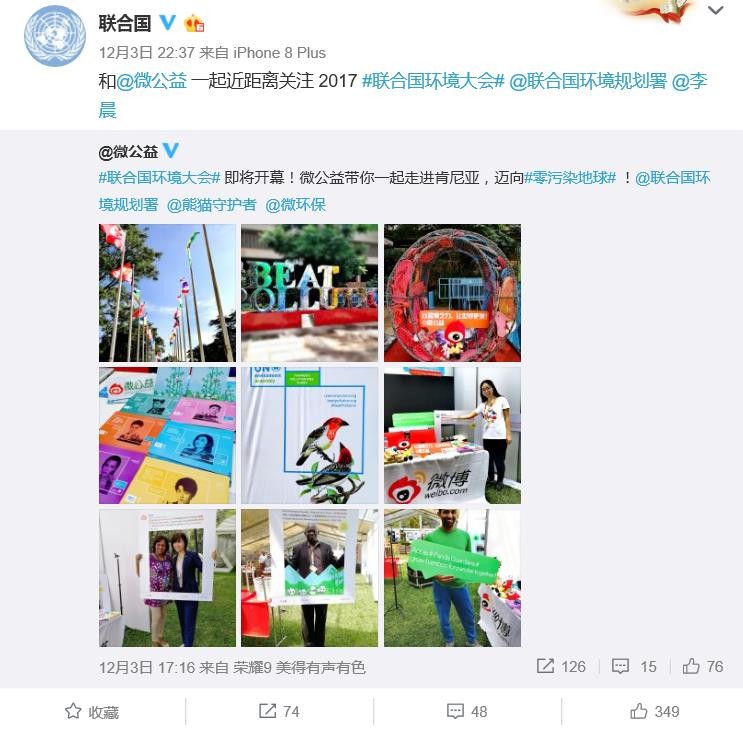
\includegraphics[width=6cm, height=4cm]{1.jpg}

            figure1
            
The four buttons under each feed are "collect, retweet, reply, like", and the capability for each button is same as twitter. When user click into the "rely" button, user can see all the comments related to the current feed, and sort them by the amount of "like" that comments get from other user. The only things differen at "weibo" is user not only can see the comments but also can see the retweet information, twitter only allow user to see who retweet the feed. Then user can see the retweet's comments and sort the list by the retweet's times of the retweet feed. So people would love to check the retweet list to see which famous person retweet the feed, and what comment they put into the retweet.Spammer control the public opinion trends by putting wrong information that doesn't represent real public opinion into the comment for some hot feed, they utilize user's habit to reach their goal. 

\section{Related work}
There are many researcher done previous research about how to distinguish the authenticity of information that post on social networking websites. Kr point out the user's social networking structure and the user's feed can represent the credible of the user, and kr using different order algorithm to rank the credible order based on the user's social networking structure and user's feed, and use it to judge the user whether is spammer or not \cite{relatd:01}. According to Liu's idea, personal information source is really important for judge the source is reliable or not, like the user register time, the user operating frequency, and the relationship between the user and comment target will be three factors for supervise fake account \cite{relatd:02}. In lou's article, he mention that we need to analysis the content and feed for judge the reliable level of information, he also point out the if only investigated the comment, retweet for detect spammer, it is hard to reach automatically fast and accuracy result, which mean it still require operator to control the analysis application \cite{relatd:03}. Xu has really unique investigate area, she investigate the spammer in online business platform, and I her idea can be work on social networking website \cite{relatd:04}. In her article, she focusing on the speciality of spammer's behavior in online business websites, she collect sixty thousand comments and thirteen thousand product information that related to those comments at Amazon, she use those data to analysis the characteristic of user behaviour and set up a classifier for different characteristic of user behaviour; she also use the relationship between different spammers to improve the level of accuracy for detecting spammer. 

\section{Method}
The method for Filtering spammer's Information at social networking websites can be divided into two part, first part is collecting data and the second part is produce data. Collecting data is the main part at this project because any analysis must base on the data, if the application can not collect the target data from third party platform, then is no way to start analysis. 

\subsection{Data Collection}
Using python 2.7 to collecting data from Weibo, and using the official SDK as my accessed method. First, setting a feed as the investigated target, I using \url{https://weibo.com/5305999252/Fy0sio7nQ?
from=page\_1005055305999252\_profile&wvr=6&mod=weibotime&type=comment} this feed to investigated the comment content. The person send this feed is my favorite gaming live streaming player, his name is LuBen Wei. He is the most popular gaming live streaming in China, there are over four million audiences what his playing game every night. Moreover, this is his second account, so he always post some feeds that can not be post at his official account at Weibo, but there are still thirty thousand comments under this feed , the number of comments at this feed even more than the comments under every signaler feed from Donald J. Trump's account. And the feed's content is he complain about the cheating case, he announced that he never cheating at "PlayerUnknown's Battlegrounds", he claim that the rumor about his cheating is come from the spammers. After he post this feed, this feed became the top 1 hot feed at the feed ranking at Webo, and most comments under this feed are abuse him cheating. So I though there are must be spammer working under this feed, the comments at a feed from a gaming live streaming player's second account is more than the comments from United states's president's feed which is so ridiculous. Therefor I think there must be spammer involved into this feed, that is how we pick up the feed which involved spammer  in social networking website. If a feed has unusual comments and likes amount compare with other feed post from the owner, that feed have huge possibility that involved spammer work. 

First of all, Weibo require we use Weibo API with authentication, so we need to create a personal application first at the weibo application apply page \cite{method:01}. Then the weibo official suggest us to use SDK to access the the API, so I came to the sdk websites \cite{method:03} to get the Weibo SDK package. Normally can just type "pip install sinaweibopy" to install this sdk package to python, and also can download the sdk package, and put the webo.py with the py files I using to collect data into the same fidder to use this sdk. I using the second method becuase I have issue pop this sdk. User can get the dirction of how to use sdk via the weibo sdk wiki page \cite{method:04}, they provide many tutorial about how to use sdk on different environment not only for pyhton.  For using Offical sdk, we need to use the "app\_key" and "app\_secret", we can find those code from the application page which I create the app apply before using my account. Those two codes are represent the user identity of who using the API, so weibo will ban the user's weibo account if they do something bad via weibo API because those two codes are directly link to user's weibo account. For getting the autorized for using the weibo API, I using Thinkgamer\_gyt's idea to get the authorized code \cite{method:05}, Weibo using OAuth 2 to check the user identity for using API. After the authorized page pump up, enter code which from the page url link which look like 
\url{https://api.weibo.com/oauth2/default.html?code=2024222384d5dc88316d21675259d73a}, and the code we need to enter is the string that after "code=" at the url link.
; then weibo will return an the access token for the API, then we using "Client" to activate the API, so we can get our target information via "Client".

After finishing open the API, the next step is to allocate the target feed page. For target the specific feed, we need to find out the id for each feed. Weibo is pretty tricky, they hide the real id and replace it as some codes at the feed URL, so we need to decode the Url to get the real feed id. 
\url{https://weibo.com/5305999252/Fy0sio7nQ?from=page_1005055305999252_profile&wvr=6&mod=weibotime&type=comment}
this link is my target feed link, take a look on the link, we can find out the the code before the question mark is pretty much look like the encryption feed id. Xuebuyuan find out the encryption rule for feed id \cite{method:02}, based on his idea, each four characters from back to front is a group as sixty binary, and switch those sixty binary to ten binary and then link them together. I using his code to decode the feed id at the ipython notebook, so user want to change their focus feed, they can enter the different codes from their focus feed's url, then they can get their feed id. 

Once we get the feed's id, we can use this id to allocate the target feed at API. The next step is to get the target information we want to analysis from the feed. We are looking for the comments information from this page, so we need to know the code about the API port for our target information. Weibo provide a API port instructions to guide the user how to access different information via API \cite{method:06}, the access port we are looking for is comment. The code of comment port can not directly use at python, then use dot instead of slash for the comment for fit the python coding rule. Then following the access port guide, setting the parameter like feed's id, the number of page we want to have for the comment, and the number of comment we want to have for each comment page. For here, I only set up return 200 comments from page one because set limited usage of API for each account, so each account only get get 2000 comments via API if the account is using free API connection, I don't want to use all the attempts chances at once. Then we use the access token which we got in the previous section to open the API and active the data port we set up for the target information. Finally set a variable to storage the data which return from the comment port.

The last step for collecting data is to storage the target data as txt file. All the data that related to comment are saved into the variable now, so if we want to get our target return object from this data set, we need to use the special code for different kind of category inside this data set; Weibo also provide a specific instruction for the code of return object \cite{method:07}. The data we need for wrong information filtration are the content of comments and the user information for each comments, the numbers of follower and the number of friends for the user who post the comments, also we need to get the number of feed that post from the user who comments the feed. Then use special code "follower\_count", "FRIENDS\_count", and "statuses\_count" to get those information, and save them into the txt file for next step data viualization. The reason why I save my target date into txt file because of the coding knowledge shortage, I don't know how to using the data analysis model at 2.7 python version, so I decide to using Python 2.7 to collecting data and using python  3.5 to do the data analysis.

\subsection{Data visualization ``'' }
The data visualization in this paper will be simple and straight forward, because of even I have some idea to analysis the data, but I can not represent it due to coding knowledge shortage. The models I decide to use for this data visualization are matplotlib, nltk, worldcloud, pandas, numpy, jieba and codecs. First, open the content.txt file at python and using readlines and appends to create a list that content all the comments. I intend to use worldcloud to visualize the words that has most frequence on the comment list, and I find out the worldcloud don't support chineses really well, so I use the module "jieba" to reproduce the comments list. Jieba is the best module to support Word Segmentation, wen can using this module to pick up the words which most frequently appear at the comment list\cite{method:08}. I using FontTian's formatting as my main structure of jieba code  \cite{method:08}, also we can add some new word into our word list and use it to make the jieb module can be able to indentity the new world, and we use "stopwords\_path" to filter the common word like "hello", and the we are using outside txt source which is Chinese vocabulary words out file as our stop word dictionary \cite{method:10}. And during using this stop word file inside the jieba code, we have to encoding the file to "utf8" formatting, otherwise it will have some error that the jieba module can not distinguish the content inside the stop word file; also we need to set up the right font for the wordcloud by using the ttc file from the fonts document on the computer, if the font use on wordcloud doesn't support chinese, the final result will be a retangle for each word instand of actually Chinese. 

The first outcome I got from the word cloud is look like this:
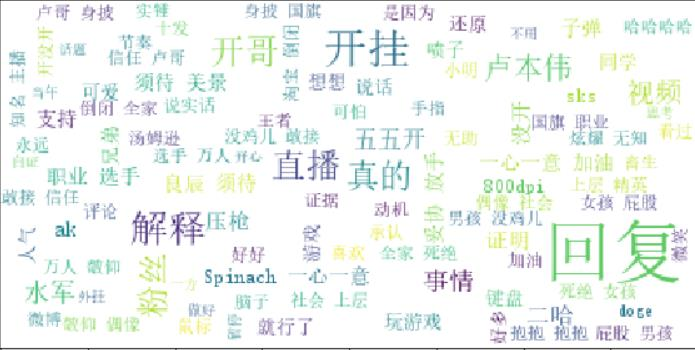
\includegraphics[width=7cm, height=4cm]{2.jpg}
So now people can really quick have a pretty idea that what is the main trend of the comments, and what is all the comment talking about. But we can still find some noise inside the plt, like ``回复'' which mean reply, it doesn't contain any meaning, so we can add this word to our stop words list, then we try to create world cloud again, the new plot is look like this:

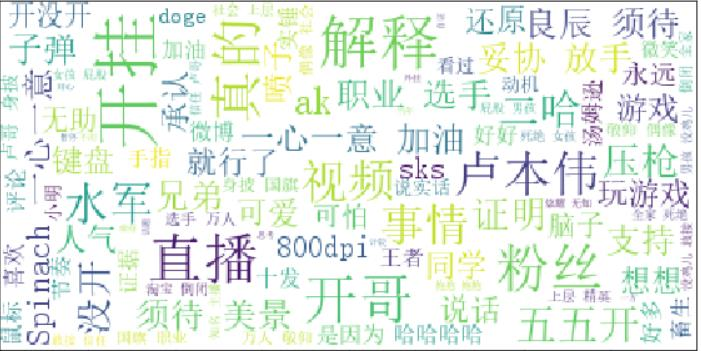
\includegraphics[width=7cm, height=4cm]{3.jpg}
It seems more meaniful than before, and contain more information than before. So we can see that their lot of words like ``回复'' inside the comments data is useless, then we can add those world into our stop words list to rip it up. Also we can use this method to filter the spammer's information, so the uesr can see the true information from the world cloud.

Then for detecting the spammer, analysis the user who post the comments is very important. To visualize the user data, using readlines to open the each txt file, and using solit and strip to reproduce the data formatting. Then putting all the data into the dataframe via pandas modules. When I look at the data type in dataframe, I found out that the data type inside the dataframe for each catory is not number, then I use astype to change the data type to number for calculator. Here is the three histograms I plot out for the the Feeds, Friends, and followers data: 

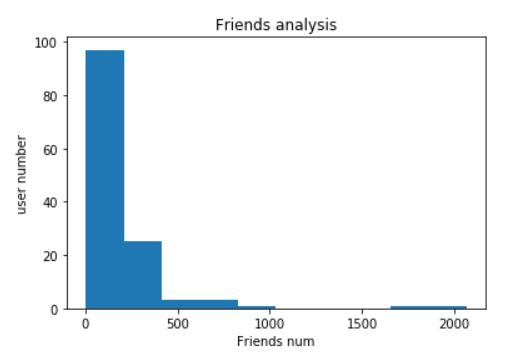
\includegraphics[width=7cm, height=4cm]{4.jpg}

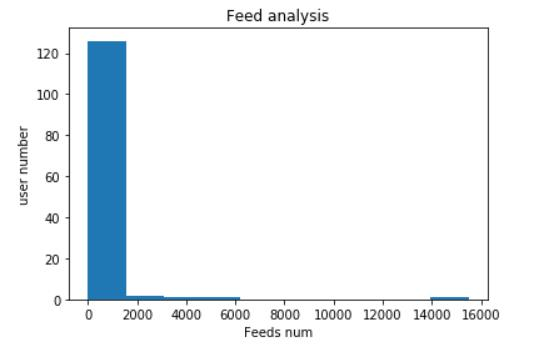
\includegraphics[width=7cm, height=4cm]{5.jpg}

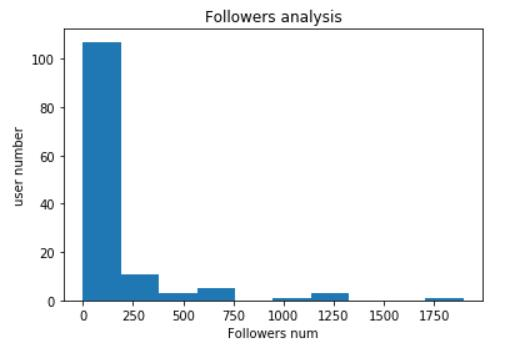
\includegraphics[width=7cm, height=4cm]{6.jpg}

The result is pretty interesting and surprise for me. The data represent those three histograms are pretty obviously, even the number of my sample is only 200 comments because of the limitation of weibo API. We can see that all the histograms are right-skewed distribution, according to the definition of histogram, the mean at right skewed distribution is the peak of the right side \cite{method:10}. It doesn't look like normal because of the curve is not bell shape, if this data is from the real commets which mean post by the actual user not spammer, the curve of this three histograms will looks like normal distribution. The peal of those three histograms show us the majority of those three elements, for the number of friends, the majority is between 0 to 250; for the majority of feeds is between 0 to 1800, and the majority for followers is between 0 to 200. we can see most majority are fall into the first interval, which mean it represent the friends, followers, and feed from the accounts I pick are pretty much same type of fake account. So it is pretty luck that I can dig out so much spammer account with small number of simple, so there no doubt that their are lot of spammers involve into this feed's comment because the comments post by the majority accounts are pretty much same type of account.




\section{Future work}
The above sections bring out the idea about how to detect the spammer, and the method is pretty sample because of it just to use for proof my idea is feasible. To rise the filter wrong information to the big data level, we can using database to storage our data instead of storage the data into a txt files. We can make a connection between API and mysql, and the programming will automatically storage the data inside each table for different data category. Also the authorized code can be automatically get from the authorized page, so user no need to enter it by hand. All the analysis will be integration into one application, so user only need to copy and paste the feed link that they want to see the true for that feed, and the application will decode the feed id and collecting all kind of data into the mysql database. For collecting huge size of data like over ten thousand comments, we can using different virtual machine to get data from the API, so we don't need to worry about the daily API usage any more.
Furthermore, using machine learning to train a model that can recognize the most frequency word that spammer use to post the wrong information, and use it the find out the spammer on the comment list. Finally, according to the comment list data analysis, save the user name which are define as spammer in database, and then remove the comments that related to those user in the comments content list, use this new comments content list to create wordcloud to represent the true trend and focus point for user's target feed. Moreover, the spammer data on the database will be cumulative, so the application analysis 
more fee, the spammer list will be increase, then each time the application can remove the comments which post by the spammer on the spammer list before analysis the spammer on the comments list which can improve the precision ratio of eliminate spammer information a lot. I think big data is based on the data precipitation, so most big data application won't have good performance at the begin because lack of data, when the application produce and save data until certain level, the performance the application  will be increase.

\section{Conclusions}
The power of social opinion not only effect the ciber world, but also have great impact on real world. Therefore, it is really important to let the user in ciber world getting right information for the content that they are interesting in; the best way to achieve this gold is using application that base on big data analysis to filtering the wrong information that post by the spammer. There lot of ways to filtering the wrong information, but the collecting related data are always same, because no matter using which way to analysis the data, getting data is top priority than any things. I believe current technology can support big data storage really well, when the data storage reach certain amount, we can use it to decontaminate the ciber world, and maintain the ciber world envirnment that allow people gain real information and create real social relationship on it. Therefore, improve the accuracy and adaptation for spammer will be meaningful to investigated. 




\section{Acknowledgement}

I would like to  take this chance to thanks to my tutor Miao, in process on reviewing my paper, he gave me many useful comments and advises. At the same time, I would like to thanks my instructor laszewsk, give me useful knowledge about how to write a report on Latex format. Finally, I would love to thanks my friends who working at IT company  give me many idea about how spammer work.


\bibliographystyle{ACM-Reference-Format}
\bibliography{report} 

\end{document}
